\subsection{Effects of Unknown Applications}
\label{sec:res:unknown}

The quality of a domain platform is also expressed in how well it supports applications unknown at design time. We explore the effect for the OpenVX domain. For this, the DSE is performed with N-1 domain applications. Throughput measurements, conversely, are performed using \newtext{the unknown application.} The process is repeated N times and results averaged. \figref{fig:unknown} reports the results.

\begin{figure}[h]
	%\vspace{-5pt}
	\centering
		\subfloat[Average Throughput Improvement]{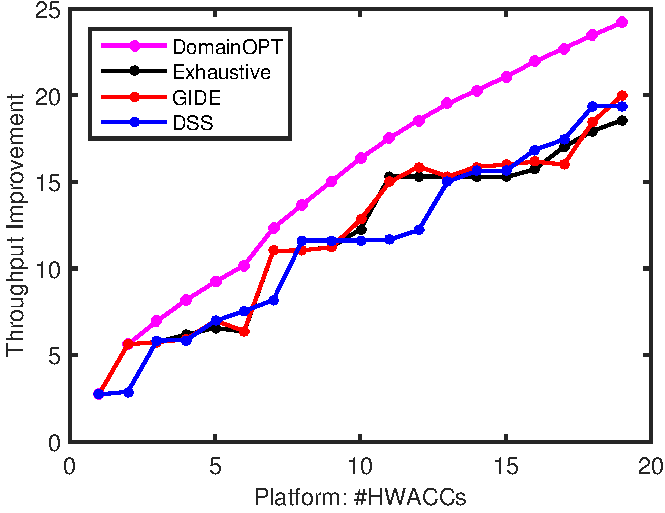
\includegraphics[width=.5\linewidth]{fig/prUnknowTh.pdf}\label{fig:unknownTh}}
		\hfill
		\subfloat[\newtext{Cumulative Performance Loss} (HW=8)]{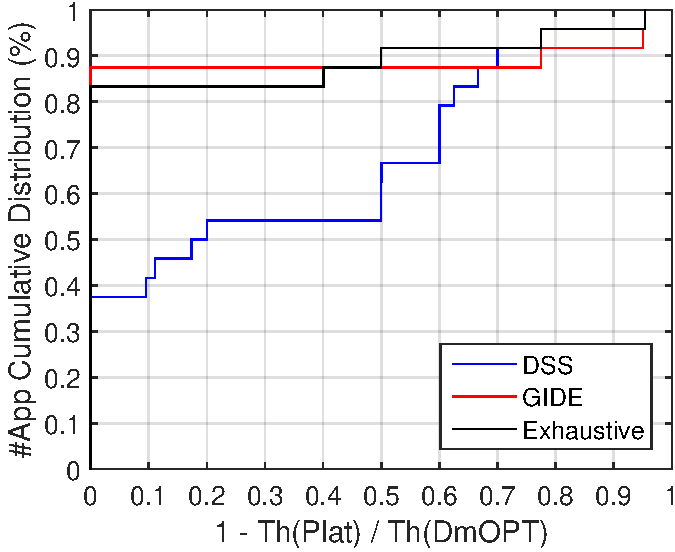
\includegraphics[width=.47\linewidth]{fig/prUnknowCD.pdf}\label{fig:unknownCD}}
	%\vspace{-8pt}
	\caption{N-1 Training, 1 Evaluation Rotating (OpenVX)}
	\label{fig:unknown}
	%\vspace{-6pt}
\end{figure}

As \figref{fig:unknownTh} shows that even the exhaustive search exhibits a significant loss over \textbf{DomainOPT} which is the oracle solution knowing all applications at design time. Comparing DSE approaches is inconsistent, as each is at least once the best due to averaging.  

\figref{fig:unknownCD} reveals much more insight showing the cumulative distribution of application throughput achievement (over DomainOPT) for a budget of 8 (where DSS had highest average improvement). 
Exhaustive and \ga show a much better distribution than DSS. In Exhaustive and \ga more than 80\% applications could achieve highest throughput. 
The reason of higher DSS average, is that DSS fully accelerate some applications which have a very high individual throughput improvement.  However, for a large size of low throughput improvement, the DSS can not accelerate it. 


%\begin{figure}[H]
%	\centering
%	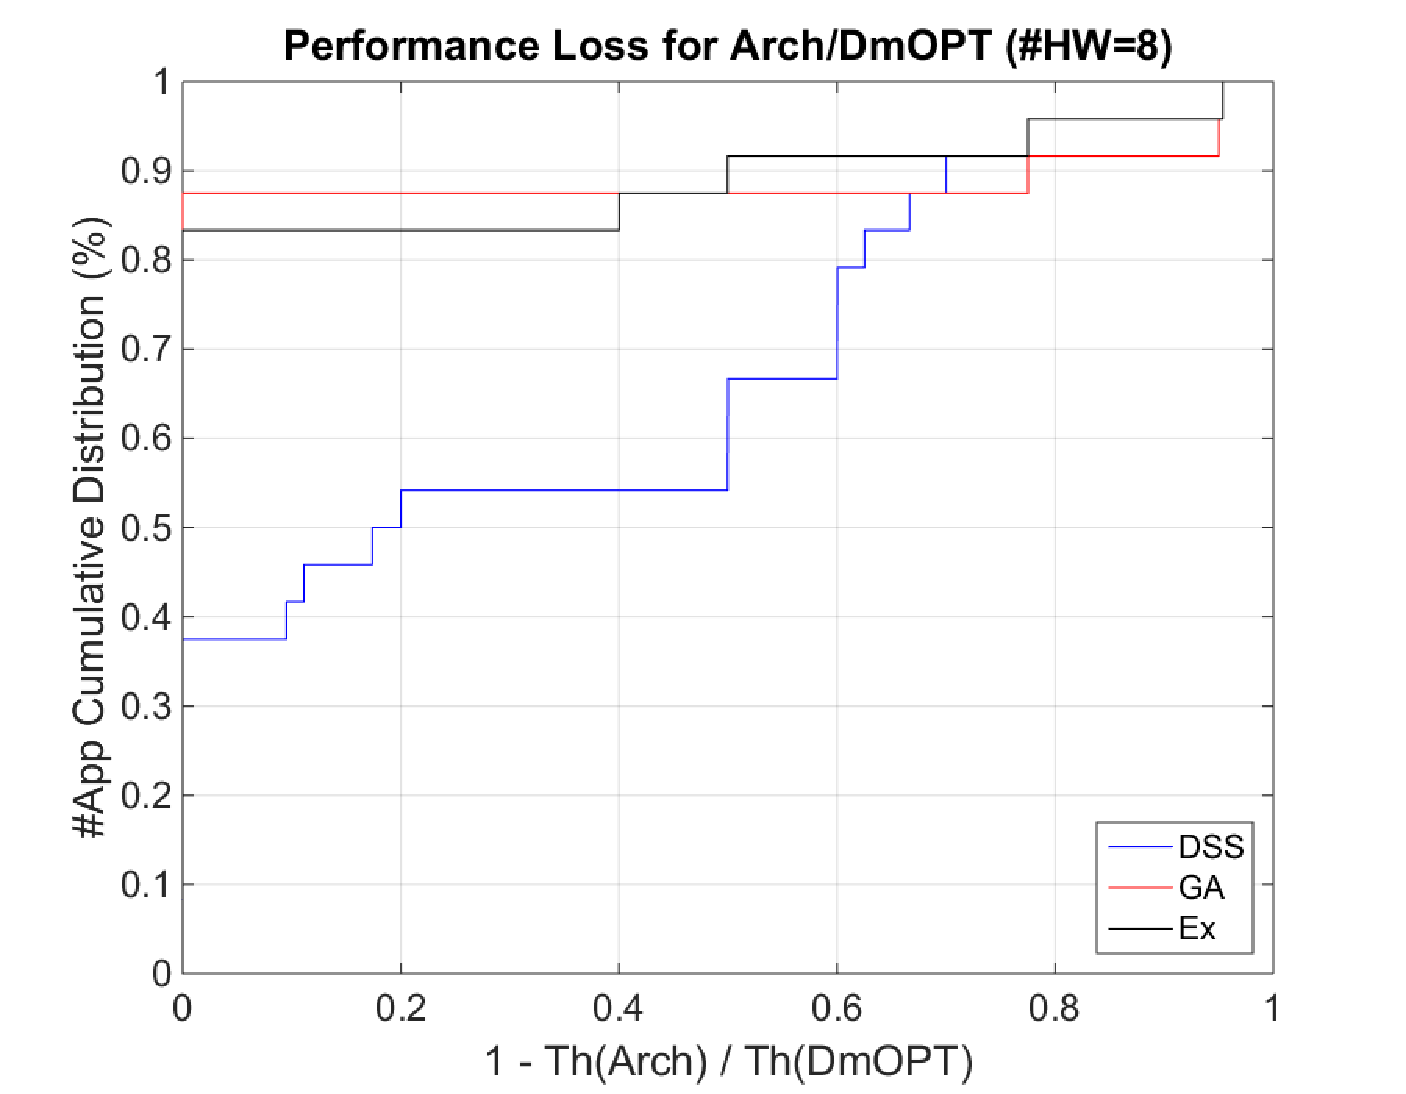
\includegraphics[width=.7\linewidth]{fig/resPerfLoss.pdf}
%	\caption{OpenVX: Throughput Loss Cumulative Distribution}
%	\label{fig:resOpenVXLoss}
%\end{figure}

%\vspace{-5pt}
\subsection{Generalization}
\label{sec:generalization}
%\vspace{-3pt}

Our analysis is best summarized as the DSE trade-off between exploration time and achieved performance. \figref{fig:paTime} quantifies the trade-off for OpenVX and synthetic domain. 


\begin{figure}[H]
	%\vspace{-5pt}
	\centering
		\subfloat[OpenVX Domain]{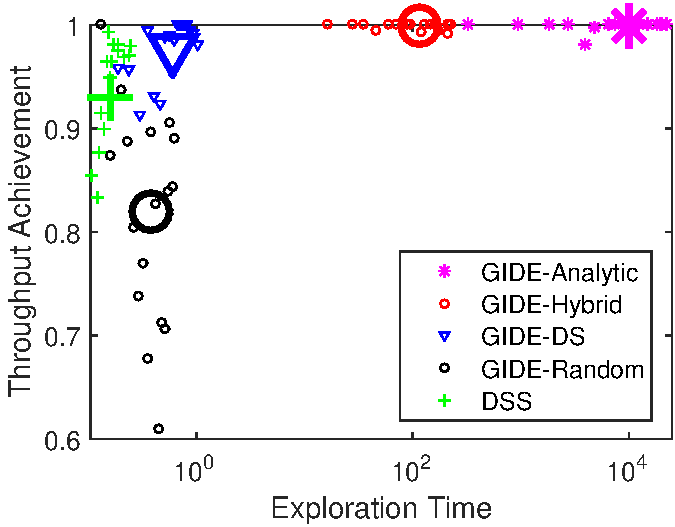
\includegraphics[width=.5\linewidth]{fig/prPATimeOpenVX.pdf}\label{fig:paTimeOpenVX}}
		\hfill
		\subfloat[Synthetic Domain]{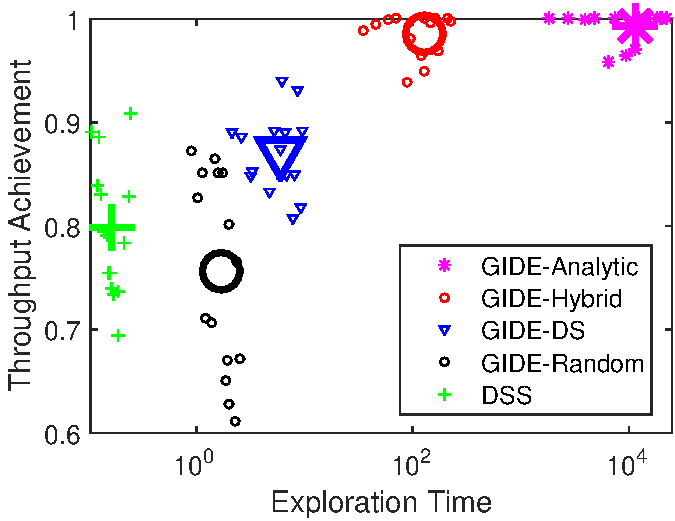
\includegraphics[width=.5\linewidth]{fig/prPATimeHWSyn.pdf}\label{fig:paTimeHWSyn}}
		%\vspace{-6pt}
	\caption{Design Exploration trade-off}
	\label{fig:paTime}
		%\vspace{-6pt}
\end{figure}

As domain size increases the trade off becomes more pronounced, i.e. it is more visible for the synthetic domain \figref{fig:paTimeHWSyn}. 
DSS achieves the fastest results but with low accuracy. \garand is similar in accuracy but much slower. DSS outperforms \garand as it uses domain features to guide the exploration. \gads produces designs with limited performance as it is limited by DS accuracy. Both \gah and \gaana approach optimal performance, while \gah is 100x faster. This makes \gah the preferred approach for DS-DSE.